% BHU PYQ -- Professional Exam Template
\documentclass[11pt,a4paper]{article}

\usepackage[a4paper,top=2.5cm,bottom=2.5cm,left=2.8cm,right=2.8cm,headheight=14pt]{geometry}
\usepackage{amsmath,amssymb}
\usepackage[T1]{fontenc}
\usepackage[utf8]{inputenc}
\usepackage{lmodern}
\usepackage{microtype}
\usepackage{fancyhdr}
\usepackage{enumitem}
\usepackage{listings}
\usepackage{hyperref}
\usepackage{lastpage}
\usepackage{parskip}
\usepackage{tikz}

\hypersetup{colorlinks=true,urlcolor=black,linkcolor=black,
  pdftitle={BVCA-202: Problem Solving AI -- BHU PYQ}}

\pagestyle{fancy}
\fancyhf{}
\renewcommand{\headrulewidth}{0.4pt}
\renewcommand{\footrulewidth}{0.4pt}
\fancyhead[L]{\small\textit{Banaras Hindu University}}
\fancyhead[R]{\small\textit{BVCA-202: Problem Solving AI}}
\fancyfoot[C]{\small Page \thepage\ of \pageref{LastPage}}

\lstset{
  basicstyle=\small\ttfamily,
  frame=single,
  breaklines=true,
  columns=flexible,
  keepspaces=true
}

\newlist{parts}{enumerate}{2}
\setlist[parts,1]{label=(\alph*),leftmargin=*,itemsep=4pt,topsep=3pt}
\setlist[parts,2]{label=(\roman*),leftmargin=*,itemsep=2pt,topsep=2pt}
\newcommand{\pts}[1]{\hfill\textit{[#1]}}

\begin{document}
\begin{center}
  {\large\bfseries BANARAS HINDU UNIVERSITY}\\[2pt]
  {\normalsize B.Voc. Semester II Examination, 2022-23}\\[6pt]
  \rule{0.8\linewidth}{0.5pt}\\[6pt]
  {\large\bfseries Paper: BVCA-202 --- Problem Solving using Artificial Intelligence}\\[4pt]
  {\normalsize Time: Three Hours \hfill Maximum Marks: 70}
\end{center}

\rule{\linewidth}{0.4pt}

\smallskip
\noindent\textit{Instructions: Section A: Attempt any 2 out of 4 questions (12 marks each). Section B: Attempt any 6 out of 9 questions (6 marks each). Section C: All questions compulsory (1 mark each).}

\bigskip

\bigskip\noindent{\large\bfseries SECTION --- A}
\rule{\linewidth}{0.4pt}\smallskip

\noindent\textit{Note: Long-answer questions to be answered in 500 words each. Attempt any 2.} \hfill \textbf{[12 $\times$ 2 = 24]}

\medskip\noindent\textbf{Question 1.} Explain different types of Agents defined based on their degree of perceived intelligence and capability.

\medskip\noindent\textbf{Question 2.} Explain how the resolution principle is used in the Prolog language by an example.

\medskip\noindent\textbf{Question 3.} Write the Best First Search algorithm. What is the difference between Greedy Best First Search versus $A^*$ Best First Search Algorithm?

\medskip\noindent\textbf{Question 4.} What do you understand by structured knowledge representation techniques? Explain any one of these techniques.

\bigskip\noindent{\large\bfseries SECTION --- B}
\rule{\linewidth}{0.4pt}\smallskip

\noindent\textit{Note: Attempt any six questions. Answer in about 200 words each.} \hfill \textbf{[6 $\times$ 6 = 36]}

\medskip\noindent\textbf{Question 5.} Give an example of any search algorithm.

\medskip\noindent\textbf{Question 6.} Explain the Hill Climbing algorithm along with its types.

\medskip\noindent\textbf{Question 7.} If horses fly or cows eat grass, then the mosquito is the national bird. If the mosquito is the national bird, then peanut butter tastes good on hot dogs. But peanut butter tastes terrible on hot dogs. Therefore, cows don't eat grass. Prove or disprove this argument using the resolution principle.

\medskip\noindent\textbf{Question 8.} Prove or disprove the validity of the following argument with respect to the given statements:
\begin{parts}
  \item If today is Tuesday then I have a test in CS or Economics.
  \item If my economics professor is sick then I will not have a test in Economics.
  \item Today is Tuesday and my economics professor is sick.
  \item \textbf{Conclusion}: Therefore, I have a test in CS.
\end{parts}

\medskip\noindent\textbf{Question 9.} Consider the following graph. Find the most cost-effective path to reach from start state $A$ to final state $J$ using the $A^*$ Algorithm:
\begin{center}
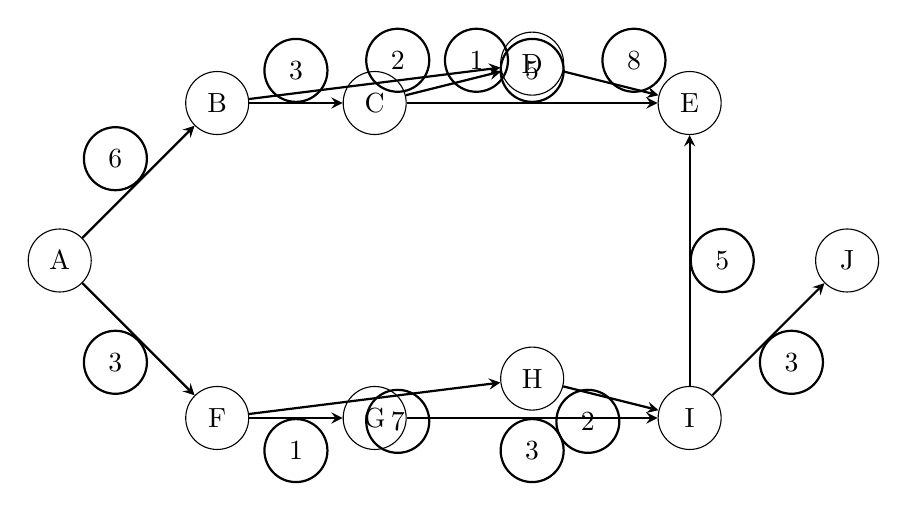
\begin{tikzpicture}[>=stealth, every node/.style={draw, circle, minimum size=8mm, inner sep=0pt}]
  \node (A) at (0,2) {A};
  \node (B) at (2,4) {B};
  \node (F) at (2,0) {F};
  \node (C) at (4,4) {C};
  \node (G) at (4,0) {G};
  \node (D) at (6,4.5) {D};
  \node (H) at (6,0.5) {H};
  \node (E) at (8,4) {E};
  \node (I) at (8,0) {I};
  \node (J) at (10,2) {J};
  \draw[->, thick] (A) -- node[above left] {6} (B);
  \draw[->, thick] (A) -- node[below left] {3} (F);
  \draw[->, thick] (B) -- node[above] {3} (C);
  \draw[->, thick] (B) -- node[above right] {2} (D);
  \draw[->, thick] (C) -- node[above right] {1} (D);
  \draw[->, thick] (C) -- node[above] {5} (E);
  \draw[->, thick] (D) -- node[above right] {8} (E);
  \draw[->, thick] (F) -- node[below] {1} (G);
  \draw[->, thick] (F) -- node[below right] {7} (H);
  \draw[->, thick] (G) -- node[below] {3} (I);
  \draw[->, thick] (H) -- node[below left] {2} (I);
  \draw[->, thick] (I) -- node[below right] {3} (J);
  \draw[->, thick] (I) -- node[right] {5} (E);
\end{tikzpicture}
\end{center}

\begin{center}
\begin{tabular}{|c|c||c|c|}
  \hline
  \textbf{Node} & \textbf{h(n)} & \textbf{Node} & \textbf{h(n)} \\
  \hline
  A & 10 & F & 6 \\
  \hline
  B & 8 & G & 5 \\
  \hline
  C & 5 & H & 3 \\
  \hline
  D & 7 & I & 1 \\
  \hline
  E & 3 & J & 0 \\
  \hline
\end{tabular}
\end{center}

\medskip\noindent\textbf{Question 10.} Write the pseudo-code for the Min-Max algorithm and explain its working with an example.

\medskip\noindent\textbf{Question 11.} Write the advantages and disadvantages of the logical representation technique of knowledge representation.

\medskip\noindent\textbf{Question 12.} Write a Prolog program to create the following knowledge base and return the answers for the queries:
\begin{parts}
  \item \textbf{Knowledge Base}:
  \begin{itemize}
    \item Mary is female.
    \item Mary is the sister of John.
    \item John is the parent of Joseph.
    \item If $x$ is female and $x$ is the sister of $z$ and $z$ is the parent of $y$, then $x$ is the aunt of $y$.
  \end{itemize}
  \item \textbf{Query}: Is Mary the aunt of Joseph?
\end{parts}

\medskip\noindent\textbf{Question 13.} Discuss the concept of rationality in AI agents. How does it relate to decision making?

\bigskip\noindent{\large\bfseries SECTION --- C}
\rule{\linewidth}{0.4pt}\smallskip

\noindent\textit{Note: Attempt all questions in a sentence each.} \hfill \textbf{[10 $\times$ 1 = 10]}

\medskip\noindent\textbf{Question 14.} Answer the following:
\begin{enumerate}[label=(\roman*),leftmargin=*,itemsep=8pt]
  \item Explain Artificial Intelligence in one sentence.
  \item What is the Turing Test?
  \item What is meant by an AI agent?
  \item Transform the following English sentence into logical notation: ``Not all integers are positive.''
  \item Transform the following English sentence into logical notation: ``Some numbers are not even.''
  \item Which of the following is not a logic programming language?
  \begin{enumerate}[label=(\alph*),itemsep=2pt]
    \item Prolog
    \item ROOP
    \item Janus
    \item C
  \end{enumerate}
  \item Which of the following is not a heuristic search?
  \begin{enumerate}[label=(\alph*),itemsep=2pt]
    \item Best First Search
    \item Hill Climbing
    \item Depth First Search
    \item A* Search
  \end{enumerate}
  \item Which of the following is not a proposition?
  \begin{enumerate}[label=(\alph*),itemsep=2pt]
    \item $X = 3$
    \item Moon is made up of cheese.
    \item $X > 6$
    \item $3 + 3 = 6$
  \end{enumerate}
  \item Which of the following is false, where the underlying universe of discourse is the set of integers?
  \begin{enumerate}[label=(\alph*),itemsep=2pt]
    \item $\forall x [x < x+1]$
    \item $\exists x [x < x+1]$
    \item $\exists x [x = x+1]$
    \item $\forall x [x = x]$
  \end{enumerate}
  \item Which of the following techniques is not a structured knowledge representation technique?
  \begin{enumerate}[label=(\alph*),itemsep=2pt]
    \item Semantic Nets
    \item Production Rules
    \item Scripts
    \item Frames
  \end{enumerate}
\end{enumerate}

\vfill
\rule{\linewidth}{0.4pt}
\begin{center}\small
\href{https://bhu-exam.vercel.app/}{Click here to visit our website}\\[4pt]\href{https://me-aryan.vercel.app/}{Click here to visit our contributor}\\[4pt]\href{https://quashan-me.vercel.app/}{Click here to visit our contributor}
\end{center}
\end{document}
